\section{Background}
\label{sec:background}

%\nancomment{
%	figures are stored in google drive, the link is pinned in slacker;
%	%https://drive.google.com/open?id=0B4jePsYXW6SSTTRLb0FHVXVjNUk
%	figures/fig-docker-architecture.pdf}\\


Virtual Machine (VM) based server virtualization technologies (\eg, VMware~\cite{vmware},
Xen~\cite{xen}, or KVM~\cite{kvm}) have been extensively used by most cloud
platforms such as Amazon EC2 as it provides strong isolation guarantees.
%
%which consists of a virtual machine monitor (VMM) on top of a host operating system.
%It supports the concurrent execution of multiple
%guest operating systems instances within virtual machines (VMs) and provide users
%with benefits ranging from application isolation through server consolidation to
%improve disaster recovery and faster server provisioning~\cite{xxx}.
%
However, they also come with high overhead in terms of CPU, memory, and I/O as
each VM requires its own operating system kernel and system calls have to go
through a privileged hypervisor. This causes long VM startup times and slows down
processing.
%
%Nevertheless,
%hypervisor-based virtualization has a high performance overhead because of execution
%time overhead caused by executing privileged instructions, specially for applications
%which relies on I/O operations and memory overhead caused by space reservation for
%the VMs buffer and various virtualization data structures.
%that allows dynamically partitioning of a machine and sharing the available physical
%resources such as CPU, storage, memory and I/O devices.
%
%\vcomment{The sentence above is 12 (!) lines long (in pdf)! We need to break it (and
%other such sentences) in several sentences.  In a scientific paper, an optimal
%sentence is of about 3 lines long and almost never longer than 6 lines (I'm talking
%about 2-column format, as used by FAST).}
%\nancomment{addressed}
%%
%\vcomment{The paragraph above might be too detailed or out-of-scope of the paper.
%Let's see how it reads later.}
%\nancomment{addressed}

%
%
%Guest OSs are normally executed at a reduced privilege level~\cite{}.
%
%Hypervisor intercepts traps from guest OSs and emulates the trapping instructions,
%which incurs execution time overheads, specially for applications which relies on
%I/O operations since I/O interrupt overhead is amplified for nested virtual machine.
%
%Memory overhead includes space reserved for the VMs buffer and various
%virtualization data structures, such as shadow page tables~\cite{}, which increases
%with the number of virtual CPUs and the configured memory for the guest OSs~\cite{}.
%
%\vcomment{First, I think we do not need to explain so much details of CPU overhead.
%
%I think for this paper it is sufficient to list overheads: memory, I/O, CPU and have
%corresponding citations.
%
%(Notice I/O and memory overheads are more prominent in hypervisor virtualization).
%
%Second, for memory overhead, we need to mention that hyperviser-based virtualization
%keeps complete copy of every guest OS in memory (compared to containers).
%
%Third, somewhere we need to state that VM start time is long (give estimates)
%(comared to containers).}
%\nancomment{addressed}


Recent container-based virtualization (such as Linux Containers~(LXC)~\cite{linux-lxc} or
OpenVZ~\cite{bibid}) has emerged as a lightweight virtualization alternative
which promises near native performance.
%
Compared to VMs, container virtualization works at the
operating system level. %and does not emulate another operating system.
%
All containers are isolated from each other but still share the same operating
system kernel. This significantly reduces overhead as less storage and memory is
required and system calls go directly to the kernel. 
%
Linux containers offer namespace isolation through
\textit{namespaces}~\cite{linux-namespaces}
while managing resources via \textit{cgroups}~\cite{linux-cgroups}.


%\vcomment{Here, we briefly need to state what are added Docker functionalities and
%benefits, rather than going into details about CoW. Basically, we need to say that
%Docker combines sofware packaging with containerization which allows bla-bla-bla.}
%\nancomment{I think these are two basic techniques for docker}
%
%Docker incorporates copy-on-write union filesystems (UnionFS) to avoid duplication
%and enable versioning.
%
%It couples the above two components with a number of features, like portability,
%re-use, and reproducibility.

%It provides a Docker CLI command line
%tool for the lifecycle management of image-based containers. Linux containers enable
%rapid application deployment, simpler testing, maintenance, and troubleshooting
%while improving security.

%, and  that make it developer-centric (and therefore distinct from traditional
%virtual machines that attempt to hew as much as possible to the metaphor of
%machine): like deployment

%AuFS (Advanced Multi-Layered Unification Filesystem) as a filesystem for
%containers. AuFS is a layered filesystem that can transparently overlay one or
%more existing filesystems. When a process needs to modify a file, AuFS creates a
%copy of that file. AuFS is capable of merging multiple layers into a single
%representation of a filesystem. This process is called copy-on-write.

%Docker using a high-level API that provides a lightweight virtualization solution
%to run processes in isolation. Docker is developed in the Go language and utilizes
%LXC, cgroups, and the Linux kernel itself. Since it��s based on LXC, a Docker
%container does not include a separate operating system; instead it relies on the
%operating system��s own functionality as provided by the underlying infrastructure.
%So Docker acts as a portable container engine, packaging the application and all
%its dependencies in a virtual container that can run on any Linux server.

% packaging and delivery technology, combining lightweight application isolation
%with the flexibility of image-based deployment methods.

%an extension of LXCs capabilities that provides higher level APIs and functionality
%as a portable container engine. It aims to improve reproducibility of applications
%by enabling bundling of container contents into a single object that can be
%deployed across machines.

%Docker is an open source project that automates the deployment of applications
%inside Linux Containers, and provides the capability to package an application
%with its runtime dependencies into a container. It provides a Docker CLI command
%line tool for the lifecycle management of image-based containers. Linux containers
%enable rapid application deployment, simpler testing, maintenance, and
%troubleshooting while improving security.

% Linux Containers LXC, a user-space control package for Linux Containers, constitute
%the core of Docker.

%Docker harnesses some powerful kernel-level technology and puts it at our fingertips.
%The concept of a container in virtualization has been around for several years, but
%by providing a simple tool set and a unified API for managing some kernel-level
%technologies, such as LXCs (LinuX Containers), cgroups and a copy-on-write
%filesystem, Docker has created a tool that is greater than the sum of its parts.
%The result is a potential game-changer for DevOps, system administrators and
%developers.

%Docker provides tools to make creating and working with containers as easy as
%possible. Containers sandbox processes from each other. For now, you can think of a
%container as a lightweight equivalent of a virtual machine.

%how container isolate.
%Docker containers create a wrapped, controlled environment on the host machine in
%which applications can be run in isolated manner via two main Linux kernel
%features -- kernel namespaces which are used to split the view that processes have
%of the system and control groups (cgroups) that restricts the resource usage of a
%process or group of processes.
%%
%Currently, Linux kernel provides six different namespaces, PID, IPC, NET, MNT,
%UTS, and USER for process IDs, IPC requests, networking, file-system mount points,
%host names, and user IDs~\cite{xxx}~\cite{xxx}.
%%
%Controlled resources include CPU shares, RAM, network bandwidth, and disk I/O.
%%
%\vcomment{This paragraph seems to belong to the Section above (on containerization)
%rather than to Docker section}.
%\nancomment{addressed}


\subsection{Docker}

Docker is a new popular container-based virtualization technology that extends LXC
with higher level APIs and additional functionality. It automates the deployment of
applications inside Linux containers, and provides the capability to package an
application with its runtime dependencies into a container.

%\vcomment{Nannan, we need to move ALL subsections to separate *.tex files.}
%\nancomment{will do it soon}
%Docker is an open platform for developers and system administrators to build, ship,
%and run distributed applications using Docker Engine, a portable, lightweight
%runtime and packaging tool, and Docker Hub, a cloud service for sharing applications
%and automating workflows. The main advantage is that,
%Docker allows packaging an application with its dependencies into a standardized,
%self-contained unit (a so-called container), which can be used for software
%development and to run the application on any system.
%Containers are an abstraction at the app layer that packages code and dependencies
%together.

\begin{figure}
	\centering
	% Requires \usepackage{graphicx}
	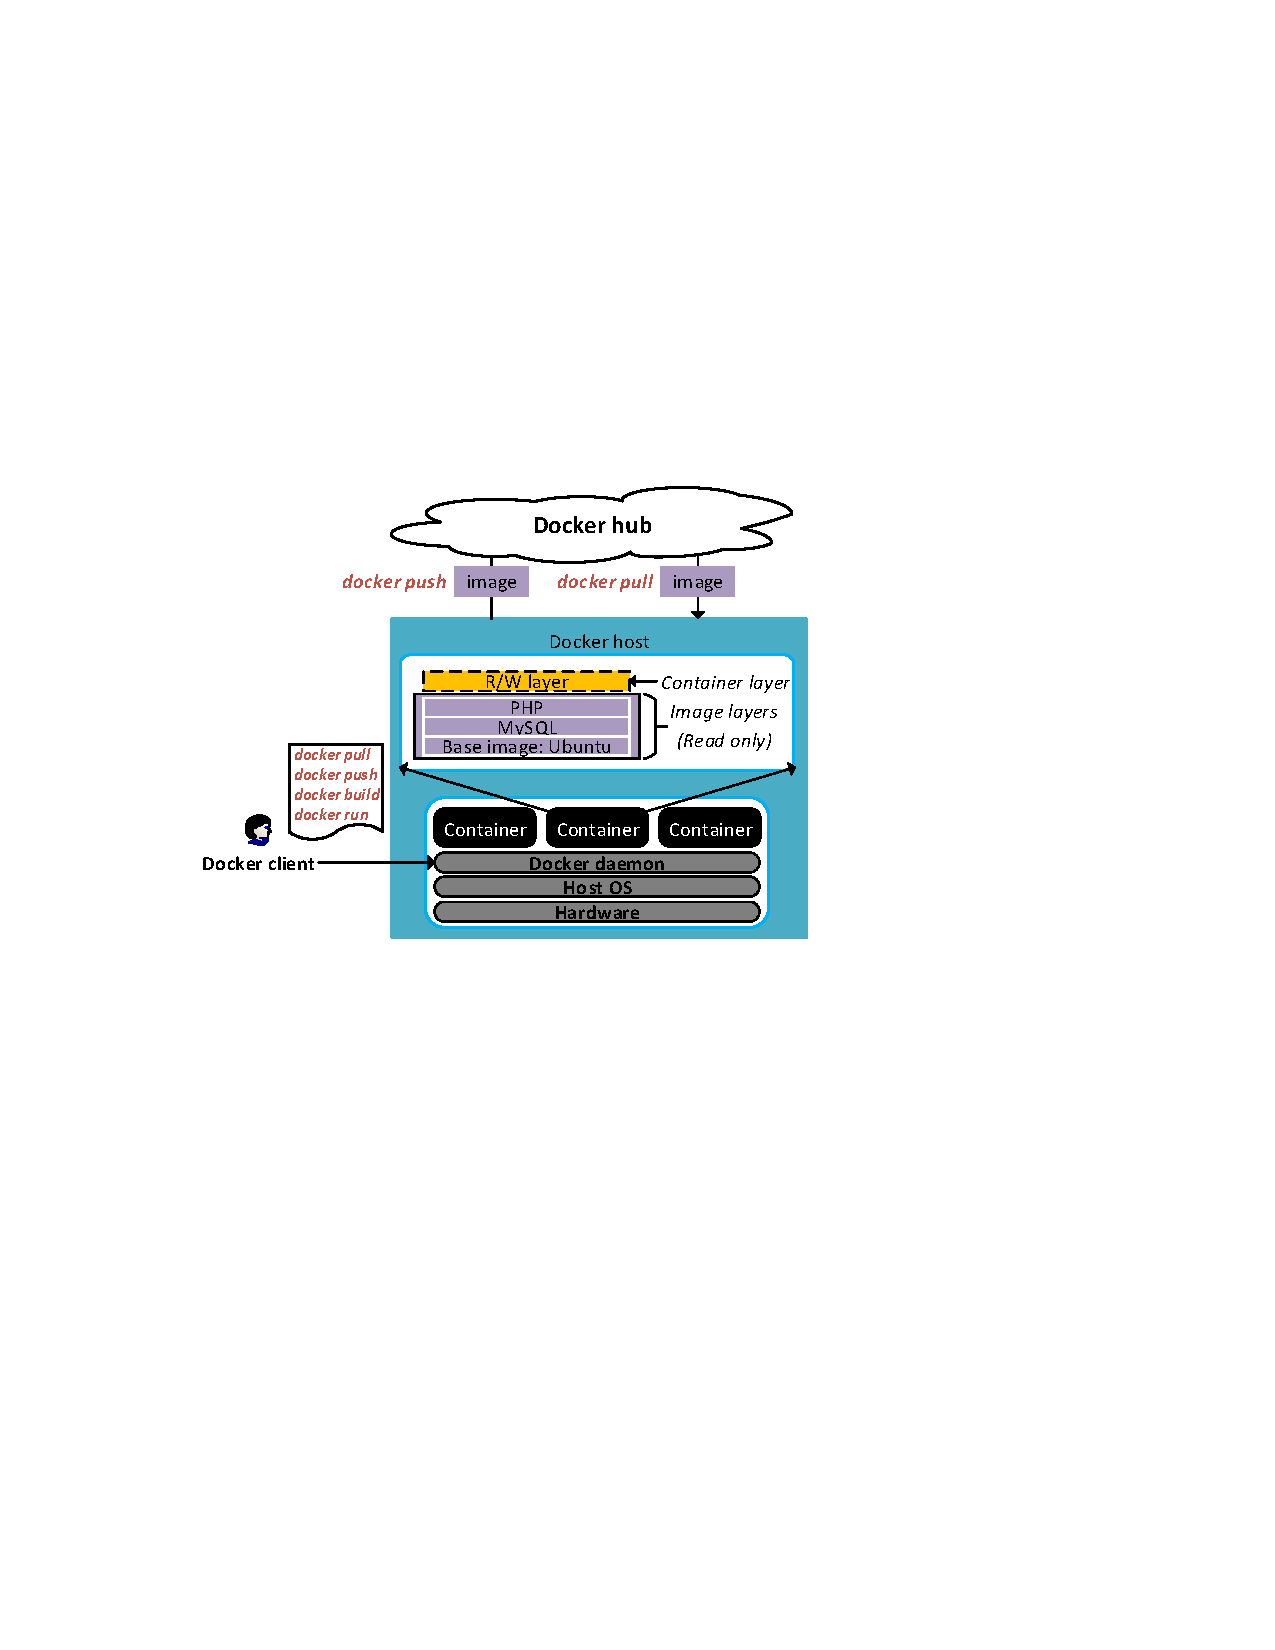
\includegraphics[width=0.5\textwidth]{graphs/fig-docker-architecture}
	\caption{Docker ecosystem \lrcomment{We need to update the figure to capture
	all the main interactions between the components and remove some unneeded
	detail, \eg official and unofficial repositories}}\label{fig-docker-architecture}
\end{figure}

As shown in Figure~\ref{fig-docker-architecture}, the Docker ecosystem consists
of a variety of components.
%i.e., Docker daemon, Docker container, Docker image, and Docker Hub.
%
Users interact with Docker via the Docker \emph{client}, which sends commands
to the Docker \emph{daemon}. The daemon is responsible for \emph{running} containers
from existing images. Additionally, the daemon supports \emph{building} new images and
\emph{pushing} them to a Docker \emph{registry}. In case a user wants to launch a
container from an image that is not available locally, the daemon will \emph{pull}
the required image from the registry.

%Docker Deamon, known as Docker engine, can create images from Dockerfiles
%(through `\textit{docker build}'), launch containers (through `\textit{docker run}'),
%and fetch non-local images from Docker registry as well as publish new images to
%Docker registry such as Docker Hub (through `\textit{docker pull}' or
%`\textit{docker push}').
%%
%It controls isolation levels of containers including cgroups, namespaces,
%capabilities restrictions, etc., and monitor them to trigger actions such as
%restart, and spawn shells into running containers for administration purposes.
%%
%\vcomment{@Nannan, I think I see the structure  you propose for this section:
%describe Docker components and their relationship using a figure. I think it is
%fine. But we desperately need the figure to write/revise this text consciously.}


%\subsection{Docker storage}

\subsection{Docker images and layers}
\label{sec-image-layers}

At the center of Docker is the concept of container images for packaging,
distributing, and running specific applications.
%
%Images are
%Docker image is an immutable and ``executable'' package that is essentially a
%snapshot of a container. Docker lunches its containers from Docker images.
%
%\vcomment{I don't think the statement above is accurate. Image is not a ``file'',
%right?}
%\nancomment{addressed.}
%
Docker images package an application with all its runtime dependencies, \eg
binaries and shared libraries.
%to maintain lightweight characteristics.
Docker images are composed of a series of individual \emph{layers}.
A layer contains a subset of the files in the image and 
usually represents a specific component/dependency of the image, \eg C library or
Java. This modular design allows layers to be shared between two containers if both
container images depend on the same component. 

%Docker images are
%composed of a series of individual layers along with metadata in the JavaScript
%Object Notation (JSON) format called manifest. Every Docker image starts from a
%base image (typically, a lightweight Linux distribution).

Image layers are read-only. However, when users start a
container via ``docker run'', Docker creates a new writable layer on top of the
underlying read-only layers. Any changes made to files in the image will be
reflected inside the writable layer via a copy-on-write mechanism. This leaves layers
unmodified throughout the lifetime of a container and enables the sharing of
layers across different containers.
Docker supports multiple storage drivers, e.g., Aufs, OverlayFS, Btrfs,
device-mapper, to efficiently combine read-only and writable layers
in a single namespace~\cite{docker-driver-eval}.
The writable layer is deleted when the container is deleted.
 

%Since each container has its own writable layer, and all changes are stored in this
%layer, multiple containers can share access to the same underlying image and yet
%have their own data state~\cite{xxx} since the underlying image is read-only copy
%of file system data. In this case, each layer contains the data modifications
%relative to the previous layer and each layer has a \textit{parent}, except for
%the base images. The base images therefore organizes the images in trees and the
%base images are the roots of trees. This structure makes the image distribution
%process more efficiently since only the modification related to a image needs to
%be distributed.

%, which are the roots of the trees.
%
%Images are read-only copies of file system data.
%
%All modifications to the container that add new or modify existing data are stored
%in a top writable layer which was initialized when a new container is created.
% All changes made to the running container
%The writable layer is deleted when the container is deleted.
%



% how to build, relation to container

%There are two methods to build an image: The first method is called interactive
%building which is carried out by starting a base image as a container (via `Docker
%run'), running commands to install the desired software on the running container,
%then committing the changes creating a new image on the local Docker
%repository~\cite{}. The second method is called building from a Dockerfile which
%is carried out by creating a Dockerfile. A Dockefile is a script file that contains
%all the commands one would normally execute manually in order to build an image.
%Dockerfile starts by loading a base image, followed by the list of Docker formatted
%commands to install the desired software. The image is built via `docker build'.

%Docker images are composed of a set of individual layers along with metadata in
%the JavaScript Object Notation (JSON) format called manifest.
%
%Each layer contains the data modifications relative to the previous layer, starting
%from a base layer/image (typically, a lightweight Linux distribution).  ``docker
%run" will add a new writable layer on top of the underlying layers for a new
%container. All changes made to the running container, such as writing new files,
%modifying existing files, and deleting files, are written to this thin writable
%layer.
%
%\vcomment{Need to exlain at which granularity are the changes maintained.}
%
%Each layer has a parent, except for the base layers/images, which are the roots of
%the trees.
%
%This structure avoid Docker pulling redundant layers.
%
%\vcomment{Explain the last sentence in a bit more details.
%
%Right now it is not clear who pulls what and why layers reduce pulling.
%
%In fact, we use ``pull'' here for the very first time.
%
%Maybe we need to explain it earlier, in Docker section.}
%\nancomment{addressed.}

%
Besides the layers, an image also contains a \emph{manifest}.
The manifest describes the various constituents of a Docker image, such as the
target hardware platform and environment settings.
%
Moreover, the manifest contains a list of layer digests for all layers required by the image.
%
%Manifests come in two schemas: older schema 1 and newer schema 2.
%
%Schema version 2 uses a config field, which references a JSON file that contains the
%configuration information.
%
%Schema version 2 also allows multi-architecture images through a \emph{fat manifest},
%which references image manifests for platform-specific versions of an image.

%\lrcomment{What about schema version 1? How are they different and why is it relevant
%for the paper?}
%
%\vcomment{I think it would be good to have here a simple figure that depicts
%relationship between image, image manifest, and layers, and how sharing of layers
%happens.}


%uses a config field references a configuration object for
% container, by digest. This configuration item is a JSON blob that the runtime uses
%to set up the container.

%The second is to move the Docker engine towards content-addressable images, by
%supporting an image model where the image��s configuration can be hashed to generate
%an ID for the image.

%The config field references a configuration object for a container, by digest. This
%configuration item is a JSON blob that the runtime uses to set up the container.

%This new schema uses a tweaked version of this configuration to allow image
%content-addressability on the daemon side.

%This second schema version has two primary goals. The first

%\begin{enumerate}
	%\item Layers.
	%\item Manifest.
	%\item Config file.
%\end{enumerate}


%\subsubsection{Docker client storage}
% what is .., benefit

%\lrcomment{TODO: shorten to one paragraph and merge with previous section}
%\vcomment{need to make sure that we talk about Docker client storage, not registry or
%anything else.}

%
%The data management of container is superintend either by Docker storage drivers
%(e.g. AUFS, OverlayFS, Btrfs, etc) or by docker data volumes.
%
%Storage driver manage container storage and mounting, which provides a view of layer
%data via a mount point that the container uses as its root file system.
%
%Storage driver usually implements copy-on-write (CoW) technique which means it does
%not update the data.
%
%Instead, storage driver creates a new copy of that part of data which is stored
%somewhere else on the disk keeping the old part as it is.
%
%\vcomment{In previous three sentences "it" is used 3 times :)
%
%It's hard to follow the logic.
%
%In general, in formal text, where possible pronouncs (it, they, etc.) should be
%avoided and actual nouns used instead.}
%\nancomment{addressed.}
%
%Docker volume is mechanism to automatically provide data persistence for containers.
%
%A volume is a directory or a file that can be mounted directly inside the container.
%
%The I/O operations through this mount path are independent of storage driver and
%executed directly on the host.



%Docker provides a variety of pluggable storage drivers that are based on Linux
%filesystem or volume manager, including advanced multi-layered unification
%filesystem (aufs), B-tree file system (Btrfs), device mapper, or OverlayFS.
%
%All of them use Copy-on-write(CoW) strategy to maximize storage efficiency.
%
%AUFS is the default storage driver for Docker container.
%Aufs and device mapper are most commonly used in modern Linux distributions
%
%\vcomment{It is not default in RHEL/CentOS, where device-mapper is the default.
%
%I think we can say
%that Aufs and DM are most commonly used in modern distributions.
%
%Notice, you also then need to adjust/remove/rewrite the sentences below.}
%\nancomment{addressed.}
%
%Aufs is a union filesystem which allows files and directories in different file
%systems to be combined and presented as a single consistent file system. 
%The modification made to an existing file is performed via copy$\_$up operation,
%which is to copy the entire file from the image layer where it exists to the
%writable container layer. The container then writes the changes to the new copy
%of the file in the container layer. Device mapper operates at the block level,
%rather than file level for maximum performance during copy-on-write (CoW)
%operations. To Update an existing file, only the relevant block of the file is
%read from the nearest layer where it exists. When the container writes the file,
%only the modified blocks are written to the container's writable layer instead of
%entire file.
%
%The unification process is referred to a union mount.
%
%AUFS can efficiently share images between multiple running containers, enabling
%fast container start times and minimal use of disk space~\cite{xxx}.

%OverlayFS (overlayer and overlay2) is a modern union filesystem that is similar to
%AUFS, but faster.

%However, CoW requires more space because it stores the old copies of data as well.

%OverlayFS layers two directories on a single Linux host and presents them as a
%single directory. These directories are called layers and the unification process
%is referred to as a union mount. OverlayFS refers to the lower directory as lowerdir
%and the upper directory a upperdir. The unified view is exposed through its own
%directory called merged. While the overlay driver only works with a single lower
%OverlayFS layer and hence requires hard links for implementation of multi-layered
%images, the overlay2 driver natively supports up to 128 lower OverlayFS layers.

%However, AUFS storage driver can introduce significant latencies into container
%write performance. This is because the first time a container writes to any file,
%the file has to be located and copied into the containers top writable layer. These
%latencies increase and are compounded when these files exist below many image layers
%and the files themselves are large.

% This capability provides better performance for layer-related Docker commands such
%as docker build and docker commit, and consumes fewer inodes on the backing
%filesystem.

%Btrfs is a next generation copy-on-write filesystem that supports many advanced
%storage technologies that make it a good fit for Docker. Btrfs is included in the
%mainline Linux kernel.  Among these features are block-level operations, thin
%provisioning, copy-on-write snapshots, and ease of administration. You can easily
%combine multiple physical block devices into a single Btrfs filesystem. btrfs
%storage driver stores every image layer and container in its own Btrfs subvolume
%or snapshot. The base layer of an image is stored as a subvolume whereas child
%image layers and containers are stored as snapshots, which only contain the
%differences introduced in that layer. The container��s writable layer is a Btrfs
%snapshot of the final image layer, with the differences introduced by the running
%container. These differences are stored at the block level.

%Device Mapper is a kernel-based framework that underpins many advanced volume
%management technologies on Linux. Docker��s devicemapper storage driver leverages
%the thin provisioning and snapshotting capabilities of this framework for image
%and container management. The devicemapper driver uses block devices dedicated to
%Docker and operates at the block level, rather than the file level. These devices
%can be extended by adding physical storage to your Docker host, and they perform
%better than using a filesystem at the level of the operating system. The
%devicemapper storage driver uses dedicated block devices rather than formatted
%filesystems, and operates on files at the block level for maximum performance
%during copy-on-write (CoW) operations. Another feature of devicemapper is its use
%of snapshots (also sometimes called thin devices or virtual devices), which store
%the differences introduced in each layer as very small, lightweight thin pools.
%Layers which are shared in common between containers are only stored on disk once,
%unless they are writable. For instance, if you have 10 different images which are
%all based on alpine, the alpine image and all its parent images are only stored
%once each on disk. Snapshots are an implenentation of a copy-on-write (CoW)
%strategy. This means that a given file or directory is only copied to the
%container��s writable layer when it is modified or deleted by that container.
%Because devicemapper operates at the block level, multiple blocks in a writable
%layer can be modified simultaneously. Snapshots can be backed up using standard
%OS-level backup utilities. Just make a copy of /var/lib/docker/devicemapper/

%Aufs is a fast reliable unification file system with some new features like
%writable branch balancing. Btrfs(B-tree file system) is a modern CoW file system
%which implements many advanced features for fault tolerance, repairand easy
%administration. Overlayfs is another modern union file system which has a simpler
%design and is potentially faster than Aufs.

%Device mapper is a Linux kernel component; it provides a mechanism for mapping
%physical block devices onto virtual block devices. These mapped devices can be
%used as logical volumes. Device mapper provides a generic way for creating such
%mappings. Device mapper maintains a table which defines device mappings. The table
%specifies how to map each range of logical sectors of the device.

% BTRFS is a Linux file system which has a poten-%tial of replacing the current
%Linux default file system,

%The start value for the first line is always zero. For other
%lines, start + length of the previous line should be equal
%to start value of the current line. Device mapper sizes are
%always specified in 512 bytes sectors. There are different
%types of mapping targets linear, striped, mirror, snapshot,
%snapshot-origin, etc.

%BTRFS (also knows as ��butter FS��) is basically a copy on write file system.
%Copy-on-write(CoW) means it does not update the data ever.[8] Instead, it creates
%a new copy of that part of data which is stored somewhere else on the disk keeping
%the old part as it is. Anyone with a decent file systems knowledge would understand
%that CoW requires more space because it stores the old copies of data as well.
%Also, it has a problem of fragmentation. Then how can a CoW file system be used
%as a default Linux file system? Wouldn��t that reduce the performance? No need
%to mention the storage space problem. Let��s dive into BTRFS to understand why
%it has become so popular.

%The primary design goal of BTRFS was to develop a generic file system which can
%perform well with any use cases and workload. Most of the file systems perform
%well for a particular specific file system benchmark, and the performance is no
%that great for other scenarios. Apart from this BTRFS also supports snapshots,
%cloning,and RAID (Level 0, 1, 10, 5, 6). This is more than any-one has bargained
%for from a file system before. One canunderstand the design complexity because
%Linux file sys-tems are deployed on all kinds of devices from computersand smart
%phones to small embedded devices.[10]The BTRFS layout is represented with B-trees,
%morelike a forest of B-trees. These are copy-on-write friendlyB-trees. As CoW
%file systems require a little more diskspace, in general, BTRFS has a very
%sophisticated mech-anism for space reclamation. It has a garbage collectorwhich
%makes use of reference counting to reclaims un-used disk space. For data integrity
%part, BTRFS usescheck sums.

%The commonly used storage drivers are

% different types

%\begin{enumerate}
%	\item aufs.
%	\item zfs.
%	\item overlay/overlay2.
%	\item devicemapper.
%\end{enumerate}

%\subsubsection{Storage driver}

% The storage driver controls how images and containers are stored and managed on
%Docker host using a pluggable architecture.

%\begin{enumerate}
%	\item aufs.
%	\item zfs.
%	\item overlay/overlay2.
%	\item devicemapper.
%\end{enumerate}

%\subsubsection{}




\subsection{Docker registry}
\label{sec:docker-registry}

Docker registry is a platform for storing and sharing container
images. Docker Hub is one of the most popular public registries,
via which users can upload, search, and download images.
%
%Users can
%also search for published images and download them through RESTful APIs with the
%Docker client.
%Furthermore,
%a storage and content delivery system, holding named Docker images, available in
%different tagged versions.
%The Docker Hub Registry is a central storage of images and 
%allows users push their Docker images to it and pulling Docker images from it.
%
%\vcomment{Docker Hub is just one instance of registry installed.
%
%I.e., Docker Registy != Docker Hub. Rephrase above.
%
%}
%
%
Registry stores images in \emph{repositories},
each containing different versions of the same image.
Docker Hub supports both public and
private repositories.
The user repositories are namespaced, that is, their name is
``$\langle namespace\rangle/\langle repository name \rangle$",
where~\textit{namespace} is the user name. While the official repositories which
are directly provided by Docker Inc. and partners are called
``$\langle repository name \rangle$".
%
%\vcomment{Somewhere we need to say that clients talk to registries using REST API.}



Docker registry stores and exchanges layers as compressed tarballs and images
as JSON-based manifests.
%
Before Docker v1.10, every image and layer was assigned a randomly generated UUID
as an identifier.
%
%\vcomment{how long was UUID?}
%\nancomment{long or short.}
%
Starting from v1.10, the Docker registry implemented a content addressable method
using an ID (also called \emph{digest}), based on a secure hash (SHA-256) of the
image and layer data.
%
%\lrcomment{Is both image and layer data used to compute hash for
%a layer?}.
%
This new method makes ID collisions highly unlikely and allows to verify data
integrity after pulling or pushing an image.
%
%\vcomment{Hashes theoretically can still collide.}
%
%\vcomment{I think we need to say which hash is used}
%\nancomment{addressed.}
%
%It also brings better sharing of layers by allowing many images to share their
%layers even if they didn't come from the same build.
%
Addressing images by their content also enables faster checks for whether a
layer is shared between two containers and whether it is already available
in local storage.
%Docker engine more easily detect
%if something has already been downloaded during a pulling to avoid pulling
%duplicate layers.
%
%\vcomment{Are the last two sentences state the same or not?}
%\nancomment{addressed. no}
%

%\lrcomment{I think we need another paragraph, describing, how images are stored
%in the registry (tarballs) and where they are stored (independently from images
%or duplicated for each image that depends on them. It would also be interesting
%to describe, how the storage driver model maps to the registry.}


%Content addressability is the foundation for the new distribution features. The
%image pull and push code has been reworked to use a download/upload manager concept
%that makes push and pull much more stable and mitigate any parallel request issues.
%The download manager also brings retries on failed downloads and better
%prioritization for concurrent downloads.

%We are also introducing a new manifest format that is built on top of the content
%addressable base. It directly references the content addressable image configuration
%and layer checksums. The new manifest format also makes it possible for a manifest
%list to be used for targeting multiple architectures/platforms (...more to come on
%that later). Moving to the new manifest format will be completely transparent.

%Because we have separated images and layers, you don't have to pull the
%configurations for every image that was part of the original build chain. We
%also don't need to create layers for the build instructions that didn't modify
%the filesystem.

%The new method gives users more security, provides a built-in way to

%The Registry is a stateless, highly scalable server side application that stores
%and lets you distribute Docker images.

%\begin{enumerate}
%	\item Registry versions.
%	\item Content addressability.
%	\item Pulling images/pushing images.
%\end{enumerate}

%\subsection{Current public registries}
